\documentclass[12pt,a4paper]{article}

\setlength{\parskip}{\baselineskip} % Increase space between paragraphs
\setlength{\parindent}{0pt} % No indentation at paragraph level

\renewcommand{\familydefault}{cmss}
\newcommand{\rp}{\textbf{Raspberry Pi}\xspace}

\usepackage{xspace}
\usepackage[ngerman]{babel} % This is needed for umlauts
\usepackage[utf8]{inputenc} % This is needed for umlauts
\usepackage[T1]{fontenc} % This is needed for correct output of umlauts in pdf
\usepackage[pdftex,breaklinks,colorlinks,
citecolor=blue,
urlcolor=blue]{hyperref}
\usepackage{graphicx}
\usepackage[german]{cleveref} % Prepend \ref with corresponding label
% Use smaller margins
\usepackage[cm]{fullpage}
\usepackage{layout}

% 'graphicx' configuration
\graphicspath{ {img/} }
\DeclareGraphicsExtensions{.jpg}

% Copy title, author to PDF metadata
\makeatletter
\AtBeginDocument{
  \hypersetup{
    pdftitle = {\@title},
    pdfauthor = {\@author}
  }
}
\makeatother

\begin{document}
% '\layout' to visualize the layout applied
\title{Raspberry Pi}
\author{Christian Ribeaud}
\maketitle

Die \rp Hardware ist ein Einplatinen Computer der von der britischen \href{https://www.raspberrypi.org/}{Raspberry Pi Foundation} gefertigt wird.

Der \rp wurde 2008 ursprünglich entwickelt, Kinder spielerisch in die Welt der Programmierung \& Elektronik einzuführen. Jedoch führte die einfache Handhabung und die fast unendlichen Möglichkeiten zu einer grossen Community, die mittlerweile durch alle Schichten und Altersklassen geht.

Der Name wird wie \textit{raspberry pie} ausgesprochen, das englische Wort für Himbeerkuchen. Die \textit{Himbeere} knüpft an die Tradition an, Computer nach Früchten zu benennen, wie etwa \textbf{Apple}. Das \textbf{Pi} stammt aus \textit{Python}, einer Programmiersprache.

Bis Februar 2017 wurden mehr als zwölf Millionen Geräte verkauft. Die Entwicklung des \textbf{Raspberry Pi} wurde mit mehreren Auszeichnungen bzw. Ehrungen bedacht. Es existiert ein großes Zubehör- und Softwareangebot für zahlreiche Anwendungsbereiche. Verbreitet ist beispielsweise die Verwendung als \href{https://www.youtube.com/watch?v=YPu7oSVbMVo}{Mediacenter}, da der Rechner Videodaten mit voller HD-Auflösung (1080p) dekodieren und über die HDMI-Schnittstelle ausgeben kann. 

\section{Anschlüsse und Komponenten}
\label{sec:comp}

Bevor man mit dem \rp richtig loslegen kann, muss man zumindest grob wissen, wo welche Anschlüsse und Komponenten liegen und für was sie gut sind. Deshalb gilt es, alle wichtigen Anschlüsse und Bauteile des \rp richtig zu identifizieren.

\subsection{Aufgabe}

Auf dem unteren Foto des \rp zeichne die folgenden Anschlüsse und Komponenten ein. Antwort befindet sich im \cref{apx:comp} (\cref{fig:rp_ls}).

\begin{figure}[h]
\centering
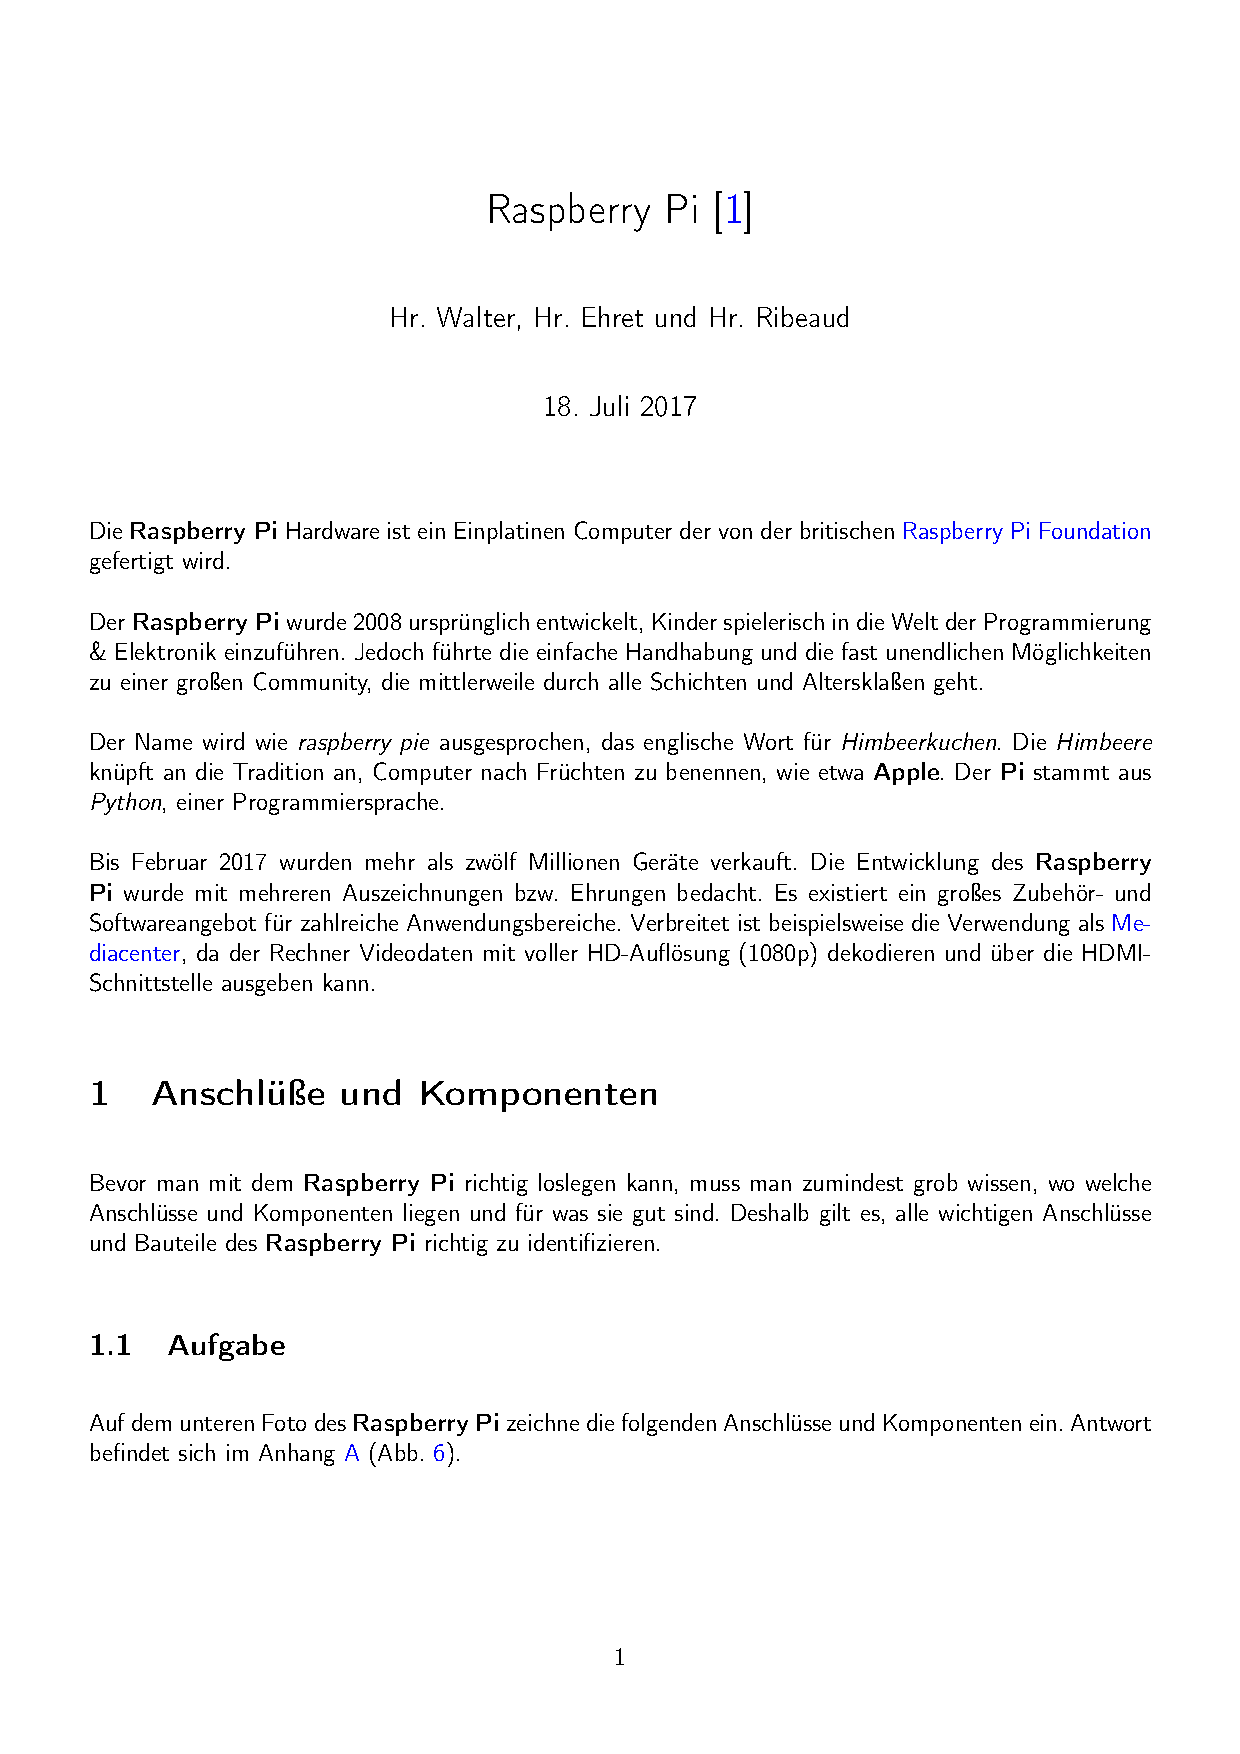
\includegraphics[scale=1.3]{raspberry}
\caption{Raspberry Pi 3}
\label{fig:rp}
\end{figure}

\begin{enumerate}
\item Wo befindet sich der Tastatur- und Maus-Anschluss (USB)?
\item Wo befindet sich der Netzwerk-Anschluss (Ethernet)?
\item Wo befindet sich der Anschluss für einen Bildschirm (HDMI)?
\item Wo befindet sich der Anschluss für Lautsprecher (Klinke)?
\item Wo befindet sich der Anschluss für die Energieversorgung (Micro-USB)?
\item Wo befindet sich der Steckplatz für die SD-Speicherkarte?
\item Wo befindet sich der Steckplatz für Erweiterungen (GPIO)?
\end{enumerate}

\section{Was man noch braucht}
\label{sec:acc}

\subsection{SD Karte}

Die \textbf{SD Karte} ist essenziell, denn das \rp kann nicht von einem USB Stick oder Festplatte gestartet werden. Der Geschwindigkeit halber wird eine Class 10 SD mit mindestens 8 GB Kapazität empfohlen. Prinzipiell sind aber bis zu 32 GB möglich. Die minimal benötigte Größe variiert von Betriebssystem zu Betriebssystem zwischen 2 und 6 GB. Falls du eine alte (micro)SD Karte aus der Kamera oder dem Handy hast, kannst du diese benutzen.

\subsection{Stromversorgung}

Damit der \textbf{Pi} genug Strom bekommt, braucht man ein microUSB Kabel mit Netzteil (gibt es auch in einem). Wenn man bereits ein microUSB Kabel hast, braucht man nur noch ein USB Netzteil, welches für den Dauerbetrieb geeignet ist und mindestens 1000mA liefert (auch diese sind separat erhältlich). Das Raspberry Pi 2/3 sollte mit einem Netzteil, welches 2000mA liefert an den Strom angeschlossen werden.

\subsection{HDMI Kabel}

Je nachdem für welche Anwendung ist ein HDMI Kabel optimal. Will man den Pi als reinen Server per SSH steuern, ist ein HDMI Kabel nicht nötig. Für andere Bereiche, wie z.B. als Multimedia Center sollte auf jeden Fall ein HDMI Kabel vorhanden sein.

\clearpage
\appendix
\makeatletter
\def\@seccntformat#1{Anhang~\csname the#1\endcsname:\quad}
\makeatother

\section{Anschlüsse und Komponenten}
\label{apx:comp}

\begin{figure}[h]
\centering
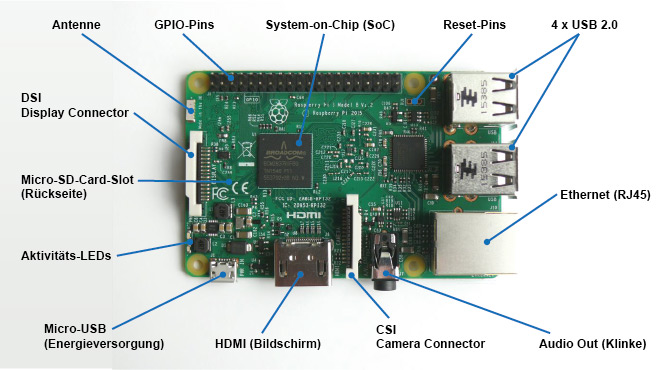
\includegraphics[scale=0.7]{raspberry_loesung}
\caption{Raspberry Pi 3}
\label{fig:rp_ls}
\end{figure}

\end{document}
